%----------------------------------------------------------------------------------------
%	PACKAGES AND OTHER DOCUMENT CONFIGURATIONS
%----------------------------------------------------------------------------------------

\documentclass{article}

\usepackage{fancyhdr} % Required for custom headers
\usepackage{lastpage} % Required to determine the last page for the footer
\usepackage{extramarks} % Required for headers and footers
\usepackage{graphicx} % Required to insert images
\usepackage{listings}
\usepackage{color}
\usepackage{xcolor}
\usepackage{caption}
\usepackage{enumitem}
\usepackage{amsmath}
\usepackage{tikz}
\usetikzlibrary{calc,shapes.multipart,chains,arrows}

\DeclareCaptionFont{white}{\color{white}}
\DeclareCaptionFormat{listing}{%
\parbox{\textwidth}{\colorbox{gray}{\parbox{\textwidth}{#1#2#3}}\vskip-4pt}}
\captionsetup[lstlisting]{format=listing,labelfont=white,textfont=white}

% Margins
\topmargin=-0.45in
\evensidemargin=0in
\oddsidemargin=0in
\textwidth=6.5in
\textheight=9.0in
\headsep=0.25in 

\linespread{1.1} % Line spacing

% Set up the header and footer
\pagestyle{fancy}
\lhead{\hmwkAuthorName} % Top left header
\chead{\hmwkClass\ (\hmwkClassInstructor\ \hmwkClassTime): \hmwkTitle} % Top center header
\rhead{\hmwkDueDate} % Top right header
\lfoot{\lastxmark} % Bottom left footer
\cfoot{} % Bottom center footer
\rfoot{Page\ \thepage\ of\ \pageref{LastPage}} % Bottom right footer
\renewcommand\headrulewidth{0.4pt} % Size of the header rule
\renewcommand\footrulewidth{0.4pt} % Size of the footer rule

\setlength\parindent{0pt} % Removes all indentation from paragraphs

%----------------------------------------------------------------------------------------
%	DOCUMENT STRUCTURE COMMANDS
%	Skip this unless you know what you're doing
%----------------------------------------------------------------------------------------

\setcounter{secnumdepth}{0} % Removes default section numbers
\newcounter{homeworkProblemCounter} % Creates a counter to keep track of the number of problems

\newcommand{\homeworkProblemName}{}
\newenvironment{homeworkProblem}[1][Problem \arabic{homeworkProblemCounter}]{ % Makes a new environment called homeworkProblem which takes 1 argument (custom name) but the default is "Problem #"
\stepcounter{homeworkProblemCounter} % Increase counter for number of problems
\renewcommand{\homeworkProblemName}{#1} % Assign \homeworkProblemName the name of the problem
\section{\homeworkProblemName} % Make a section in the document with the custom problem count
}

%----------------------------------------------------------------------------------------
%   COLORS AND LANGUAGAGE
%----------------------------------------------------------------------------------------

\lstset{
    frame=lrb,xleftmargin=\fboxsep,xrightmargin=-\fboxsep,language=Java,basicstyle=\ttfamily,
    breaklines=true,columns=fullflexible,keepspaces=true,escapeinside={\%*}{*)}
       }

%----------------------------------------------------------------------------------------
%	NAME AND CLASS SECTION
%----------------------------------------------------------------------------------------

\newcommand{\hmwkTitle}{Homework\ \#1} % Assignment title
\newcommand{\hmwkDueDate}{Wednesday,\ January\ 28,\ 2015} % Due date
\newcommand{\hmwkClass}{COP\ 5621} % Course/class
\newcommand{\hmwkClassTime}{6:25pm} % Class/lecture time
\newcommand{\hmwkClassInstructor}{Smith} % Teacher/lecturer
\newcommand{\hmwkAuthorName}{Musa V. Ahmed \& Jose Acosta} % Your name

%----------------------------------------------------------------------------------------

\begin{document}
\belowcaptionskip=-10pt

%----------------------------------------------------------------------------------------
%	PROBLEM 1
%----------------------------------------------------------------------------------------

\begin{homeworkProblem}
    Implemented a simple program analyzer and interpreter for the straight-line programming
    language. This exercise serves as an introduction to \emph{environments} (symbol tables
    mapping variable names to information about the variables); to \emph{abstract syntax}
    (data structures representing the phrase structure of programs); to \emph{recursion over
    tree data structures}, useful in many parts of a compiler; and to a \emph{functional style}
    of programming without assignment statements.
    \vspace{5 mm}

    \hspace{4 mm}It also serves as a "warm-up" exercise in Java programming. Programmers experienced in
    other languages but new to Java should be able to do this exercise, but will need
    supplementary material (such as textbooks) on Java. 

    \hspace{4 mm}Programs to be interpreted are already parsed into abstract syntax, as described by the
    data types in Program 1.5.

    \hspace{4 mm}However, we do not wish to worry about parsing the language, so we write this program by
    applying data constructors:

    \begin{lstlisting}[frame=none]
    Stm prog = 
    new CompoundStm(new AssignStm("a",
                        new OpExp(new NumExp(5)m
                                    OpExp.Plus, new NumExp(5),
                                                OpExp.Plus, new NumExp(3)))m
    new CompoundStm(new AssignStm("b",
        new EseqExp(new PrintStm(new PairExpList(new IdExp("a"),
                    new LastExpList(new OpExp(new IdExp("a"),
                                    OpExp.Minus,new NumExp(1))))),
                                    
            new OpExp(new NumExp(10), OpExp.Times,
                        new IdExp("a")))),
    new PrintStm(new LastExpList(new IdExp("b"))));
    \end{lstlisting}

    Files with the data type declarations for the trees, and this sample program, are available
    in the directory \verb!$MINIJAVA/chap1!.

    \hspace{4 mm}Writing interpreters without side effects (that is, assignment statements that update
    variables and data structures) is a good introduction to \emph{denotational semantics} and
    \emph{attribute grammars}, which are methods for describing what programming languages do.
    It's often a useful technique in writing compilers, too; compilers are also in the business
    of saying what programming languages do.

    \hspace{4 mm}Therefore, in implementing these programs, never assign a new value to any variable or
    object field except when it is initialized. For local variables, use the initializing form
    of declaration (for example, \verb!int i=j+3;!) and for each class, make a constructor
    function (like the \verb!CompoundStm! constructor in Program 1.5).

    \begin{enumerate}
        \item Write a Java function \verb!int maxargs(Stm s)! that tells the maximum number of
            arguments of any \verb!print! statement within any subexpression of a given
            statement. For example, \verb!maxargs(prog)! is 2.

        \item Write a Java function \verb!void interp(Stm s)! thats "interprets" a program in
            this language. To write in a "functional programming" style - in which you never
            use an assignment statement - initialize each local variable as you declare it.
    \end{enumerate}

    \hspace{4 mm}Your function that examine each \verb!Exp! will have to use \verb!instanceof! to determine
    which subclass the expression belongs to and then cast to proper subclass. Or you can add
    methods to the \verb!Exp! and \verb!Stm! classes to avoid the use of \verb!instanceof!.

    \hspace{4 mm}For part 1, remember that print statements can contain expressions that contain other print
    statements.

    \hspace{4 mm}For part 2, make two mutually recursive functions \verb!interpStm! and \verb!interpExp!.
    Represent a "table," mapping identifiers to the integer values assigned to them, as a list
    of \verb!id! x \verb!int! pairs.

    \begin{lstlisting}[frame=none]
    class Table {
        String id; int value; Table tail;
        Table(String i, int v, Table t) {id=i; value=v; tail=t;}
    }
    \end{lstlisting}

    Then \verb!interpStm! is declared as

    \begin{lstlisting}[frame=none]
    Table interpStm(Stm s, Table t)
    \end{lstlisting}

    taking a table $t_1$ as argument and producing the new table $t_2$ that's just like $t_1$
    except that some identifiers map to different integers as a result of the statement.

    \hspace{4 mm}For example, the table $t_1$ thats maps $a$ to 3 and maps $c$ to 4, which we
    write $\{a \mapsto 3, c \mapsto 4\}$ in mathematical notations, could be represented as the
    linked list
    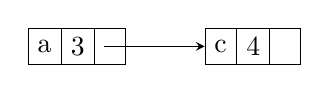
\begin{tikzpicture}[list/.style={rectangle split, rectangle split parts=3,
        draw, rectangle split horizontal}, >=stealth, start chain]

        \node[list, on chain] (A) {
            \nodepart{one} {a}
            \nodepart{two} {3}
            \nodepart{three} {}
        };
        \node[list, on chain] (B) {
            \nodepart{one} {c}
            \nodepart{two} {4}
            \nodepart{three} {}
        };
        \draw[->] let \p1 = (A.three), \p2 = (A.center) in (\x1,\y2) -- (B);

    \end{tikzpicture}.

    \hspace{4 mm}Now, let the table $t_2$ be just like $t_1$, except that is maps $c$ to 7
    instead of 4. Mathematically, we could write,

    \hspace{4 mm}$t_2$ = update($t_1$, $c$, 7),

    where the update function returns a new table $\{a \mapsto 3, c \mapsto 7\}$.

    \hspace{4 mm}On the computer, we could implement $t_2$ by putting a new cell at the headof
    the linked list: 

    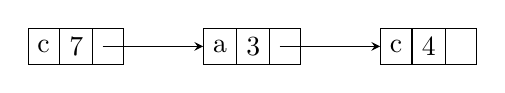
\begin{tikzpicture}[list/.style={rectangle split, rectangle split parts=3,
        draw, rectangle split horizontal}, >=stealth, start chain]

        \node[list, on chain] (A) {
            \nodepart{one} {c}
            \nodepart{two} {7}
            \nodepart{three} {}
        };
        \node[list, on chain] (B) {
            \nodepart{one} {a}
            \nodepart{two} {3}
            \nodepart{three} {}
        };
        \node[list, on chain] (C) {
            \nodepart{one} {c}
            \nodepart{two} {4}
            \nodepart{three} {}
        };
        \draw[->] let \p1 = (A.three), \p2 = (A.center) in (\x1,\y2) -- (B);
        \draw[->] let \p1 = (B.three), \p2 = (B.center) in (\x1,\y2) -- (C);
    \end{tikzpicture}, as long as we assume that the \emph{first} occurrence of $c$ in the lsit
    takes precedence over any later occurrence.

    \hspace{4 mm}Therefore, the \verb!update! function is easy to implement; and the
    corresponding \verb!lookup! function

    \begin{lstlisting}[frame=none]
    int lookup(Table t, String key)
    \end{lstlisting}

    just searches down the linked list. Of course, in an object-oriented style \verb!int
    lookup(String key)! should be a method of the \verb!Table! class.

    \hspace{4 mm}Interpreting expressions is more complicated than interpreting statements,
    because expressions return integer values \emph{and} have side effects. We wish to simulate
    the straight-line programming language's assignment statements without doing any side
    effects in the interpreter itself. (The \verb!print! statements will be accomplished by
    interpreter side effects, however.) The solution is to declare \verb!interpExp! as 

\end{homeworkProblem}
\clearpage

%----------------------------------------------------------------------------------------

\end{document}
